% ============================================================
%  CHƯƠNG 6: QUẢN TRỊ HỆ THỐNG (ADMIN)
%  Phụ trách: [Trưởng nhóm] -- TODO: điền Họ tên + MSSV
%  Packages: ui/admin (AdminActivity, dashboard, review, moderators,
%            profile), utils/Role, utils/SessionManager
%  Models:   data/model/admin/{DashboardStats, AdminPost,
%            ModeratePostRequest, PostModerationHistoryItem,
%            Moderator, AddModeratorRequest, UpdateModeratorStatusRequest,
%            ModeratorActionHistoryItem}, data/model/post/PostStatus
%  API:      data/remote/AdminApiService
%  Ghi chú: File này được \input{} từ main.tex
% ============================================================

\chapter{Quản trị hệ thống}

Chương này trình bày phân hệ quản trị và kiểm duyệt của ứng dụng Trọ Tốt:
phân quyền cho cán bộ kiểm duyệt, bảng điều khiển thống kê, duyệt/từ chối tin
đăng, theo dõi lịch sử kiểm duyệt, quản lý kiểm duyệt viên và hồ sơ quản trị.
Toàn bộ phân hệ viết bằng \tech{Java} theo kiến trúc MVVM thống nhất với các
chương trước: tầng giao diện (Activity/Fragment) quan sát \code{LiveData} do
ViewModel phát ra, ViewModel gọi Repository, Repository gọi server qua
\tech{Retrofit} trên luồng \tech{RxJava3} và bọc kết quả vào \code{Resource<T>}
(ba trạng thái \code{LOADING}/\code{SUCCESS}/\code{ERROR}). Phụ thuộc được tiêm
bằng \tech{Hilt}. Khác với người dùng thường, cán bộ kiểm duyệt sau khi đăng
nhập được đưa vào một Activity riêng (\code{AdminActivity}) thay vì
\code{MainActivity}, tạo ranh giới rõ ràng giữa hai khu vực của ứng dụng.

% ============================================================
\section{Tổng quan chức năng quản trị}
% ============================================================

\subsection{Vai trò và phân quyền trong hệ thống}
Hệ thống định nghĩa ba vai trò trong lớp \code{utils/Role}: \code{Customer}
(người dùng thường -- người thuê hoặc chủ trọ), \code{Moderator} (kiểm duyệt
viên) và \code{Manager} (quản lý). Vai trò được server cấp khi tạo tài khoản và
nhúng vào \tech{JWT}; phía ứng dụng, \code{SessionManager.getRole()} bóc tách
trường \code{roleName} từ payload token (Base64) để biết tài khoản đang đăng
nhập thuộc nhóm nào -- không tin vào dữ liệu rời rạc có thể bị thiếu.

Trên cơ sở vai trò, ứng dụng phân hai mức quyền:
\begin{itemize}
    \item \code{isAdminUser()} -- đúng với \code{Moderator} hoặc \code{Manager}:
    được vào khu quản trị (bảng điều khiển và duyệt tin).
    \item \code{isManager()} -- chỉ đúng với \code{Manager}: thêm được các quyền
    quản lý kiểm duyệt viên.
\end{itemize}
Việc kiểm tra quyền ở client chỉ nhằm ẩn/hiện giao diện cho hợp lý; server vẫn
là nơi chốt chặn cuối cùng -- mọi endpoint quản trị đều được backend kiểm tra
phạm vi quyền trước khi xử lý.

\subsection{Điều hướng theo vai trò và giao diện quản trị}
Ngay sau khi xác định phiên đăng nhập, ứng dụng rẽ nhánh theo vai trò:
\code{SplashActivity} (mở app khi đã có phiên) và \code{AuthActivity} (vừa đăng
nhập xong) đều gọi \code{sessionManager.isAdminUser()} để quyết định mở
\code{AdminActivity} hay \code{MainActivity}, kèm cờ
\code{FLAG\_ACTIVITY\_CLEAR\_TASK} để xóa back stack. Luồng rẽ nhánh được mô tả
ở Hình~\ref{fig:c6_role_routing}.

\begin{figure}[H]
    \centering
    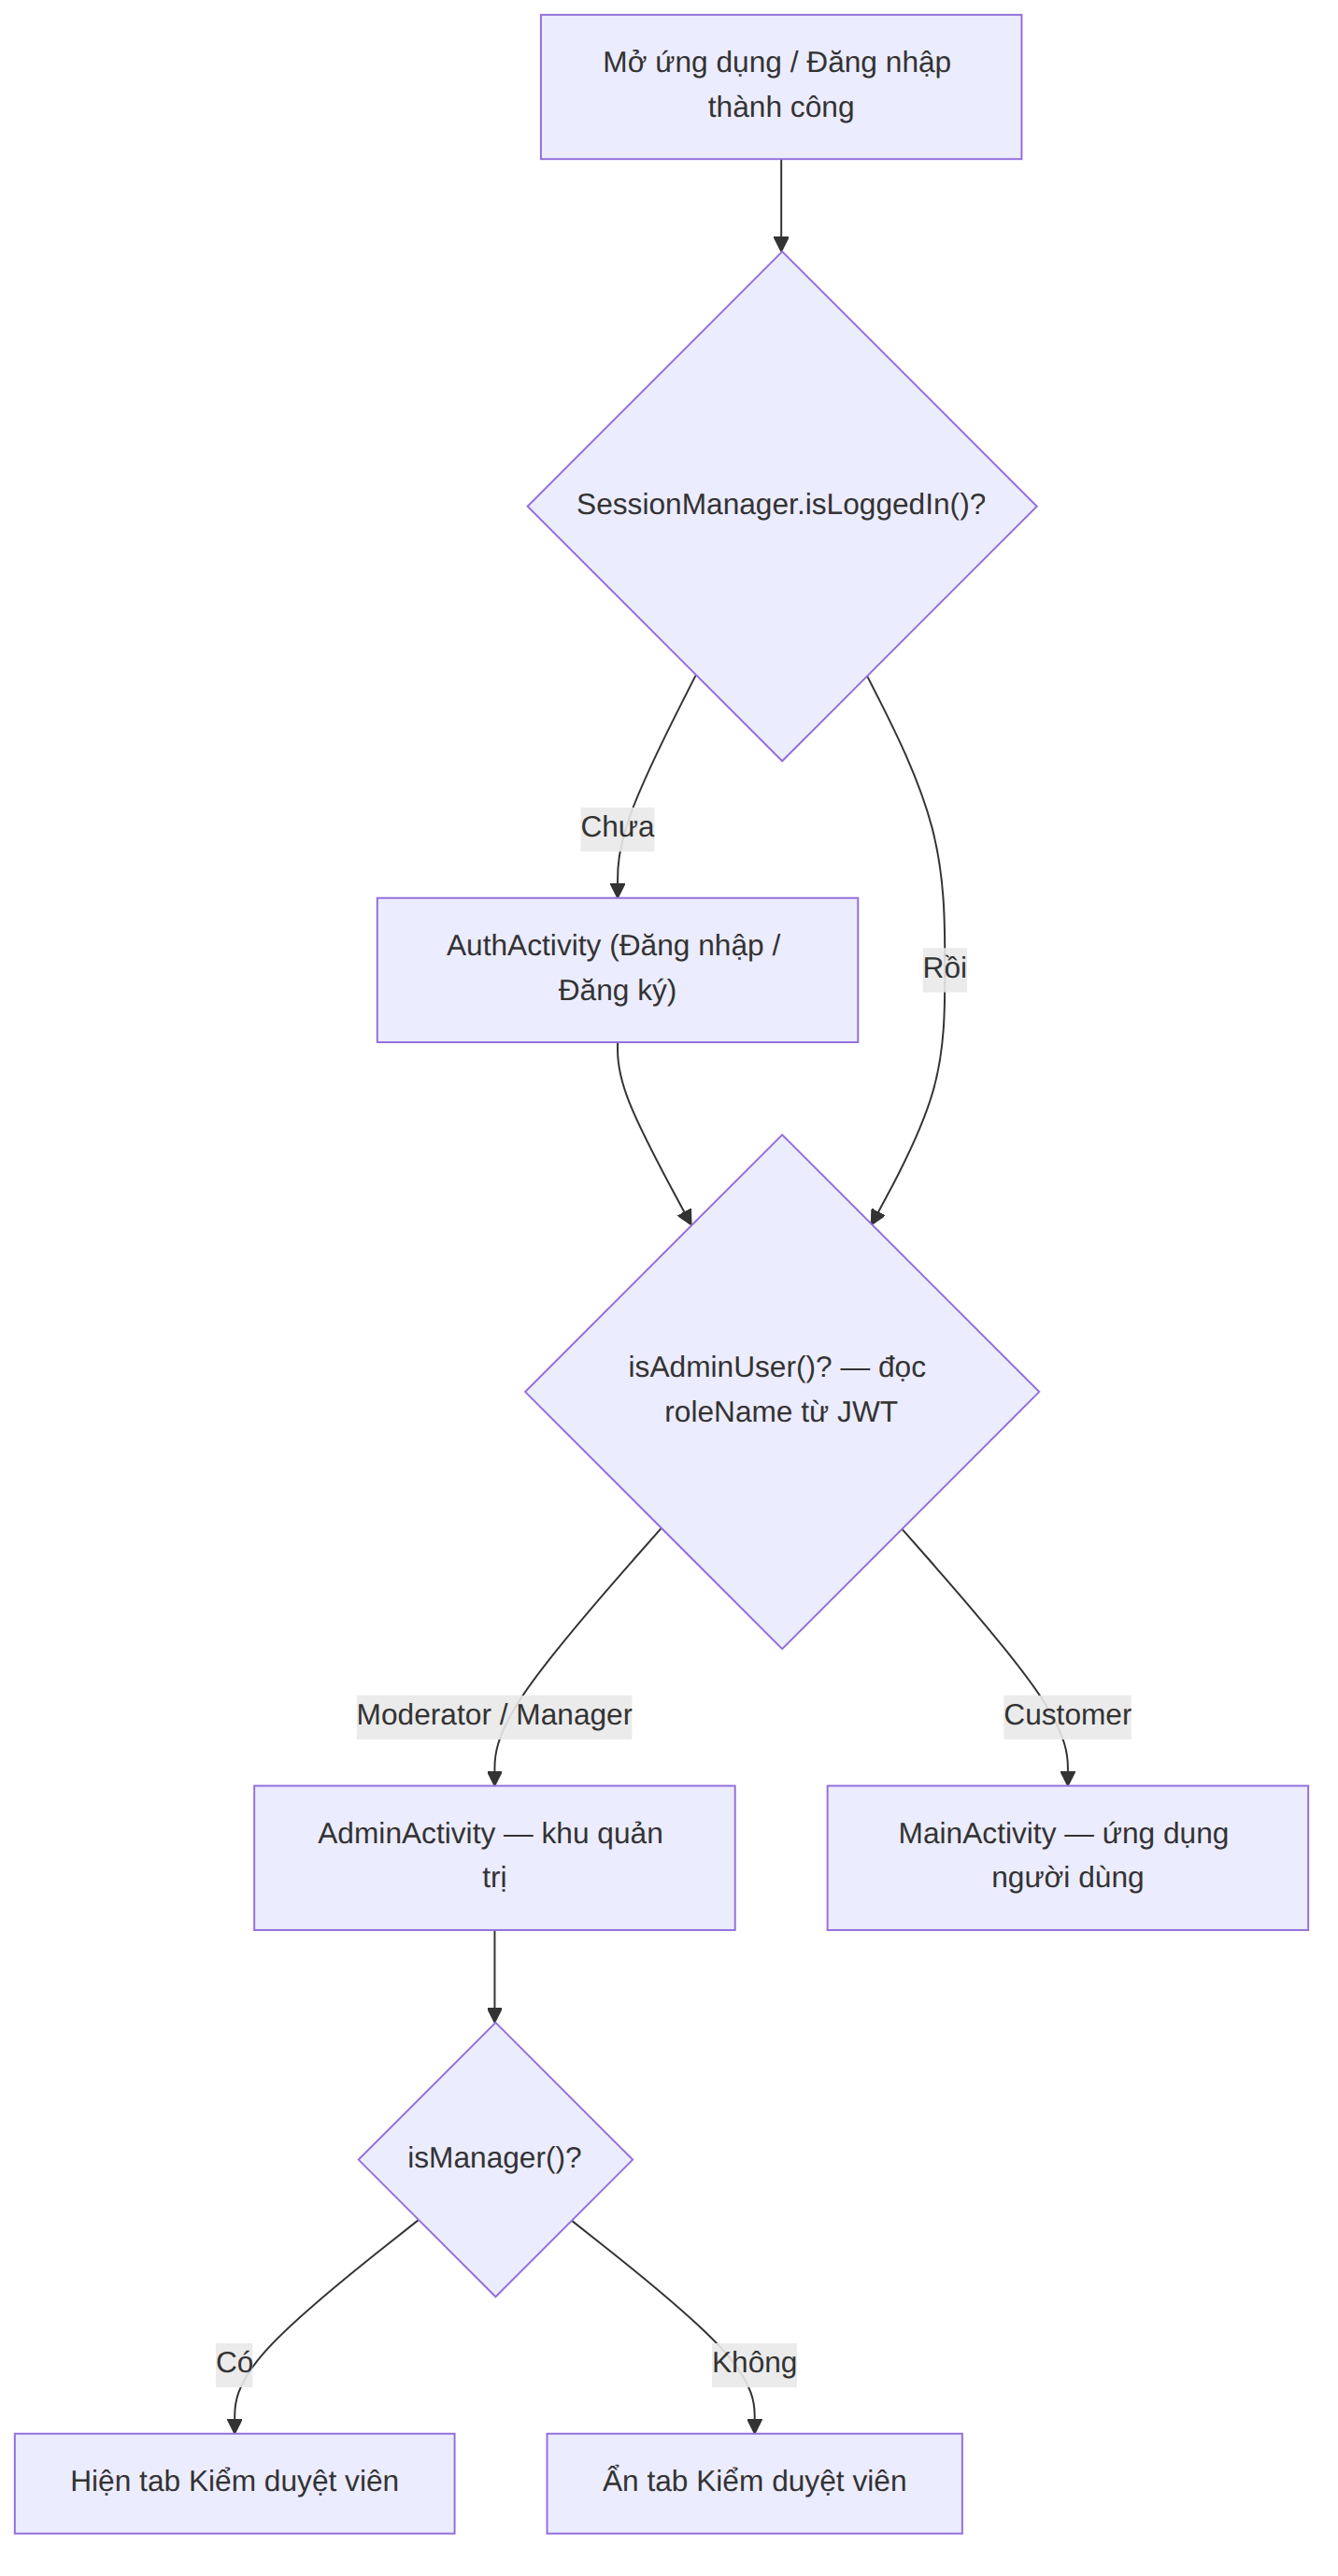
\includegraphics[width=0.62\textwidth]{images/outputs/c6_role_routing.png}
    \caption{Điều hướng theo vai trò khi khởi động và sau đăng nhập}
    \label{fig:c6_role_routing}
\end{figure}

Khu quản trị nằm trong \code{AdminActivity} (\code{@AndroidEntryPoint}). Activity
này host một \code{NavHostFragment} chạy đồ thị điều hướng
\code{admin\_nav\_graph} và gắn với một \code{BottomNavigationView} gồm bốn mục:
\screen{Tổng quan}, \screen{Duyệt tin}, \screen{Kiểm duyệt viên} và \screen{Hồ
sơ}. Phương thức \code{applyRoleVisibility()} ẩn mục \screen{Kiểm duyệt viên}
đối với tài khoản không phải \code{Manager}, nên một kiểm duyệt viên thường chỉ
thấy ba mục. \code{NavigationUI.setupWithNavController()} đồng bộ thanh điều
hướng với đồ thị, giúp chuyển màn hình mà không cần tạo Activity riêng cho từng
chức năng.

\textit{Đáp ứng CLO2: phân quyền theo vai trò (Customer / Moderator / Manager),
tách biệt khu quản trị với khu người dùng và ẩn/hiện chức năng theo quyền.}

% ============================================================
\section{Bảng điều khiển (Dashboard)}
% ============================================================

\subsection{Yêu cầu chức năng}
Màn hình đầu tiên của khu quản trị cung cấp một cái nhìn nhanh về khối lượng
công việc kiểm duyệt: số tin đang chờ duyệt, số tin đã duyệt và số tin đã từ
chối trong tuần. Kiểm duyệt viên không cần thao tác gì -- mở lên là thấy số
liệu, có thể vuốt để làm mới.

\subsection{Thiết kế giao diện}
Layout \code{fragment\_admin\_dashboard.xml} đặt nội dung trong
\code{NestedScrollView}, bọc bởi \code{SwipeRefreshLayout} để kéo làm mới:
\begin{itemize}
    \item Ba \code{MaterialCardView}, mỗi thẻ chứa \code{TextView} hiển thị một
    chỉ số: tin chờ duyệt (\code{tvPendingCount}), đã duyệt trong tuần
    (\code{tvApprovedCount}) và đã từ chối trong tuần (\code{tvRejectedCount}).
    \item Một biểu đồ cột \code{BarChart} của thư viện \tech{MPAndroidChart} so
    sánh trực quan số tin đã duyệt và đã từ chối trong tuần (cột xanh -- đỏ).
    \item \code{ProgressBar} báo trạng thái tải lần đầu.
\end{itemize}

% TODO: Bỏ comment sau khi chụp màn hình và lưu ảnh vào images/outputs/
% \begin{figure}[H]
%     \centering
%     \includegraphics[width=0.4\textwidth]{images/outputs/c6_dashboard.png}
%     \caption{Bảng điều khiển quản trị}
%     \label{fig:c6_dashboard}
% \end{figure}

\subsection{Luồng xử lý}
\begin{enumerate}
    \item \code{AdminDashboardFragment} khởi tạo biểu đồ, đăng ký observe
    \code{statsLiveData} rồi gọi \code{viewModel.loadStats()}.
    \item \code{AdminDashboardViewModel} phát \code{Resource.loading()} và gọi
    \code{adminRepository.getDashboardStats()}.
    \item Repository gửi \code{GET api/admin/dashboard-stats} trên luồng IO, ánh
    xạ phản hồi thành \code{Resource<DashboardStats>} rồi trả về Main Thread.
    \item Thành công, Fragment đổ ba con số vào các thẻ và vẽ lại biểu đồ qua
    \code{updateChart()}; lỗi thì hiện \code{Toast} thông báo.
\end{enumerate}

\subsection{Triển khai trên Android}
\begin{itemize}
    \item \textbf{Lớp chính:} \code{AdminDashboardFragment},
    \code{AdminDashboardViewModel} (\code{@HiltViewModel}) thuộc package
    \code{ui/admin/dashboard}.
    \item \textbf{API sử dụng:} \code{GET api/admin/dashboard-stats}
    $\rightarrow$ \code{DashboardStats\{totalPendingPost,
    totalApprovedPostInWeek, totalRejectedPostInWeek\}}.
    \item \textbf{Thư viện:} \tech{MPAndroidChart} cho biểu đồ cột.
\end{itemize}

\textit{Đáp ứng CLO2: tổng hợp dữ liệu từ server và trực quan hóa bằng biểu đồ
phục vụ công tác quản trị.}

% ============================================================
\section{Kiểm duyệt bài đăng}
% ============================================================

\subsection{Yêu cầu chức năng}
Mọi tin đăng mới của chủ trọ đều ở trạng thái chờ duyệt và chỉ hiển thị công
khai sau khi được kiểm duyệt viên thông qua. Tại khu quản trị, kiểm duyệt viên
xem danh sách tin chờ duyệt, mở chi tiết từng tin (thông tin, hình ảnh, người
đăng) rồi quyết định \screen{Duyệt} hoặc \screen{Từ chối}. Khi từ chối, lý do
là bắt buộc và có thể kèm đánh dấu \screen{nội dung vi phạm} để phục vụ thống
kê. Toàn bộ luồng được tóm tắt ở Hình~\ref{fig:c6_moderation_flow}.

\begin{figure}[H]
    \centering
    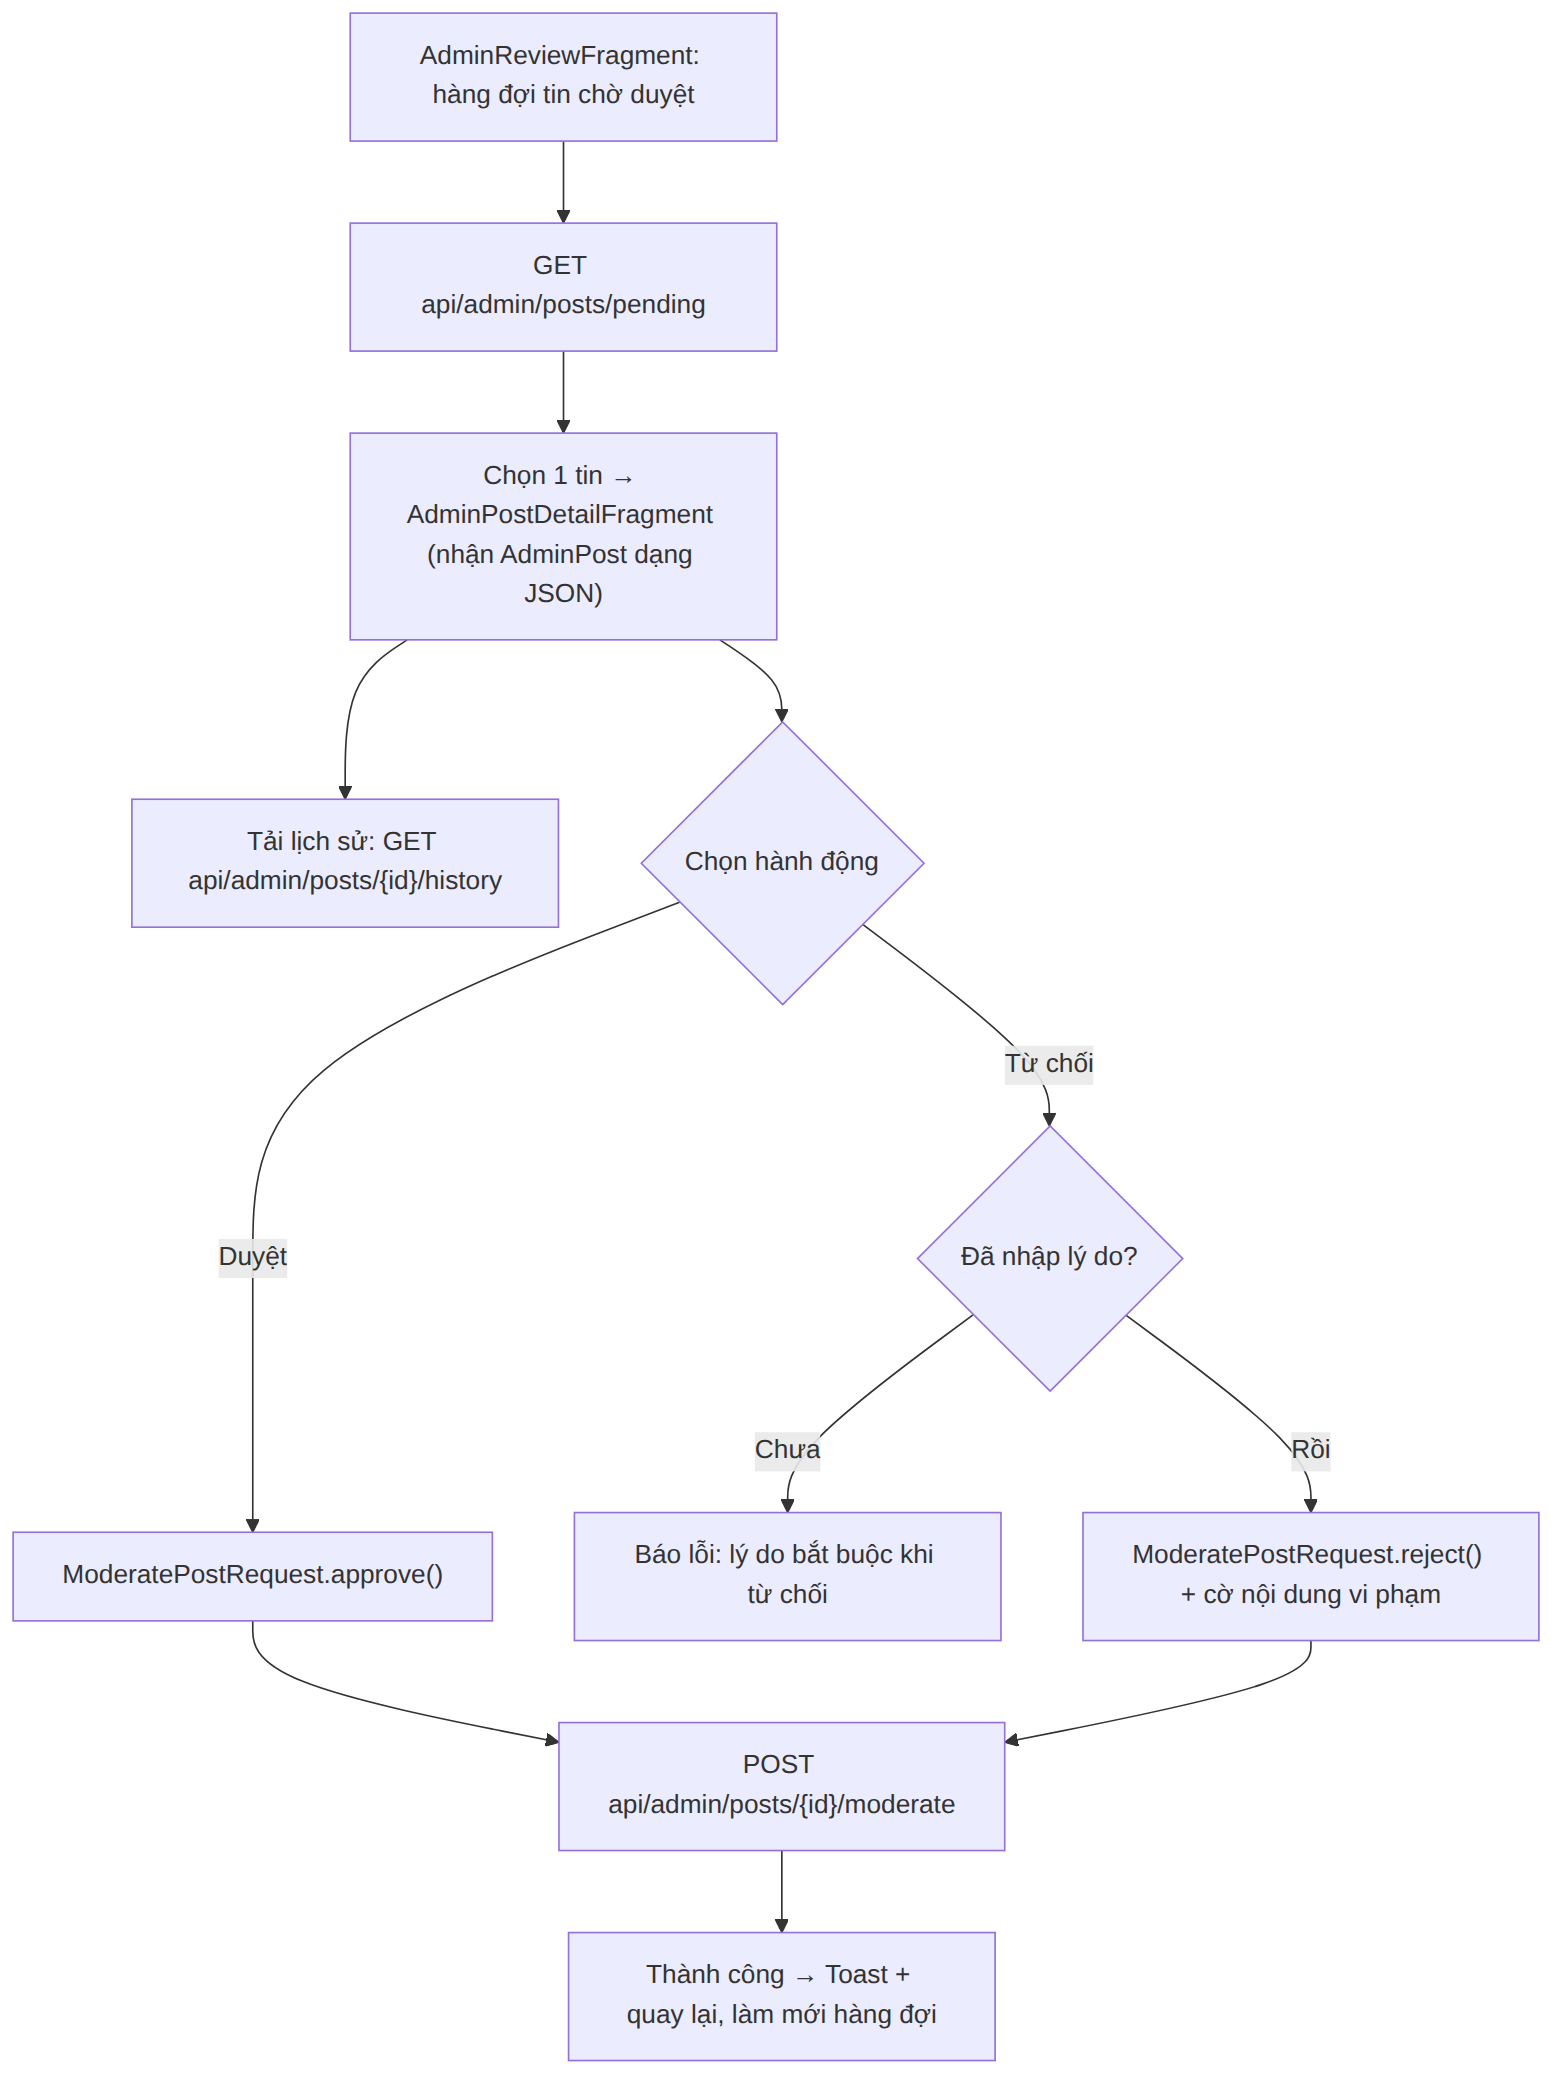
\includegraphics[width=0.72\textwidth]{images/outputs/c6_moderation_flow.png}
    \caption{Luồng kiểm duyệt một bài đăng}
    \label{fig:c6_moderation_flow}
\end{figure}

\subsection{Thiết kế giao diện}
Màn hình hàng đợi (\code{AdminReviewFragment}, layout
\code{fragment\_admin\_review.xml}) dùng \code{RecyclerView}
(\code{rvPendingPosts}) với \code{AdminPendingPostAdapter} -- mỗi dòng là một
\code{MaterialCardView} hiển thị ảnh đại diện, tiêu đề, giá và khu vực; kèm
\code{SwipeRefreshLayout} và \code{TextView} thông báo rỗng (\code{tvEmpty}).

Màn hình chi tiết (\code{AdminPostDetailFragment}, layout
\code{fragment\_admin\_post\_detail.xml}) gồm:
\begin{itemize}
    \item \code{RecyclerView} ngang trình chiếu thư viện ảnh (tái sử dụng
    \code{PostImageAdapter} của màn hình xem tin) và các \code{TextView} hiển
    thị tiêu đề, giá, diện tích, địa chỉ, mô tả, thông tin chủ tin.
    \item \code{MaterialButtonToggleGroup} với hai nút \screen{Duyệt} /
    \screen{Từ chối}; \code{TextInputLayout} + \code{TextInputEditText} nhập lý
    do; \code{MaterialCheckBox} (\code{cbHate}) \screen{Đánh dấu nội dung vi
    phạm} -- chỉ hiện khi chọn từ chối.
    \item \code{MaterialButton} gửi quyết định (\code{btnSubmit}),
    \code{ProgressBar} trạng thái và một \code{RecyclerView} lịch sử kiểm duyệt
    (trình bày ở mục~\ref{sec:c6_history}).
\end{itemize}

% TODO: Bỏ comment sau khi chụp màn hình và lưu ảnh vào images/outputs/
% \begin{figure}[H]
%     \centering
%     \includegraphics[width=0.4\textwidth]{images/outputs/c6_review_queue.png}
%     \caption{Hàng đợi tin chờ duyệt}
%     \label{fig:c6_review_queue}
% \end{figure}
% \begin{figure}[H]
%     \centering
%     \includegraphics[width=0.4\textwidth]{images/outputs/c6_post_detail.png}
%     \caption{Màn hình duyệt chi tiết một tin}
%     \label{fig:c6_post_detail}
% \end{figure}

\subsection{Luồng duyệt và từ chối tin}
\begin{enumerate}
    \item \code{AdminReviewFragment} gọi \code{loadPendingPosts()} trong
    \code{onResume()} -- vừa tải lần đầu, vừa tự làm mới khi quay lại từ màn
    hình chi tiết. Repository gọi \code{GET api/admin/posts/pending}.
    \item Người dùng chạm một dòng; Fragment truyền tin đăng sang màn hình chi
    tiết dưới dạng chuỗi \tech{JSON} (Gson) trong \code{Bundle} -- backend không
    có endpoint lấy tin chờ duyệt theo \code{id} nên dữ liệu được mang theo
    sẵn.
    \item Màn hình chi tiết bind dữ liệu, nạp lịch sử kiểm duyệt theo
    \code{postId} và đặt mặc định nút \screen{Duyệt}.
    \item Khi bấm gửi: nếu là \screen{Từ chối} mà ô lý do trống, hiển thị lỗi
    ngay tại \code{TextInputLayout} và dừng lại. Ngược lại, Fragment dựng
    \code{ModeratePostRequest} tương ứng.
    \item \code{AdminPostDetailViewModel.moderate()} gọi
    \code{POST api/admin/posts/\{postId\}/moderate}.
    \item Thành công: hiện \code{Toast} (\screen{Đã duyệt bài đăng} hoặc
    \screen{Đã từ chối bài đăng}) và \code{navigateUp()} về hàng đợi -- danh
    sách tự làm mới nên tin vừa xử lý biến mất.
\end{enumerate}

Đoạn mã dưới đây là điểm đáng lưu ý của \code{ModeratePostRequest}: lý do khi
duyệt là tùy chọn, nhưng nếu gửi chuỗi rỗng thì backend (ràng buộc
\code{@minLength(1)}) sẽ trả lỗi 400. Vì vậy hàm \code{blankToNull()} chuyển
chuỗi trống thành \code{null} để Gson bỏ qua trường này khi gửi.

\begin{lstlisting}[caption={Dựng yêu cầu kiểm duyệt -- chuẩn hóa lý do trống về null}, label={lst:c6_moderate}]
public static ModeratePostRequest approve(String reason) {
    return new ModeratePostRequest(ACTION_APPROVED, blankToNull(reason), false);
}

public static ModeratePostRequest reject(String reason, boolean isHateContent) {
    return new ModeratePostRequest(ACTION_REJECTED, blankToNull(reason), isHateContent);
}

private static String blankToNull(String s) {
    return (s == null || s.trim().isEmpty()) ? null : s;
}
\end{lstlisting}

\subsection{Các trạng thái bài đăng (PostStatus)}
Vòng đời một tin đăng được mô tả bằng \code{enum PostStatus} (package
\code{data/model/post}), khớp với chuỗi trạng thái phía backend. Kết quả kiểm
duyệt ở trên chính là yếu tố chuyển tin từ \code{PENDING} sang \code{APPROVED}
hoặc \code{REJECTED}. Các giá trị được tổng hợp ở Bảng~\ref{tab:c6_poststatus}.

\begin{table}[H]
    \centering
    \caption{Các trạng thái của bài đăng}
    \label{tab:c6_poststatus}
    \begin{tabular}{ll}
        \toprule
        \textbf{Trạng thái} & \textbf{Ý nghĩa} \\
        \midrule
        \code{PENDING}  & Mới đăng, đang chờ kiểm duyệt \\
        \code{APPROVED} & Đã duyệt, hiển thị công khai \\
        \code{REJECTED} & Bị từ chối kèm lý do \\
        \code{EXPIRED}  & Hết hạn hiển thị \\
        \code{HIDDEN}   & Đã bị ẩn khỏi danh sách công khai \\
        \bottomrule
    \end{tabular}
\end{table}

\subsection{Triển khai trên Android}
\begin{itemize}
    \item \textbf{Lớp chính:} \code{AdminReviewFragment},
    \code{AdminReviewViewModel}, \code{AdminPostDetailFragment},
    \code{AdminPostDetailViewModel} thuộc package \code{ui/admin/review}.
    \item \textbf{API sử dụng:} \code{GET api/admin/posts/pending}
    $\rightarrow$ \code{List<AdminPost>}; \code{POST
    api/admin/posts/\{postId\}/moderate} với body
    \code{ModeratePostRequest\{actionType, reason, isHateContent\}}.
\end{itemize}

\textit{Đáp ứng CLO1 và CLO2: luồng duyệt/từ chối tin hoàn chỉnh với
RecyclerView, validation lý do và gọi API qua Retrofit.}

% ============================================================
\section{Lịch sử kiểm duyệt}
\label{sec:c6_history}
% ============================================================

\subsection{Yêu cầu chức năng}
Để bảo đảm minh bạch và truy vết được trách nhiệm, mỗi bài đăng lưu lại lịch sử
các lần kiểm duyệt: hành động (duyệt/từ chối), lý do, thời điểm và người thực
hiện. Ngoài ra, quản lý có thể xem lịch sử hành động của từng kiểm duyệt viên
để đánh giá hoạt động.

\subsection{Thiết kế giao diện}
Lịch sử kiểm duyệt của một bài hiển thị ngay trong màn hình chi tiết qua
\code{RecyclerView} (\code{rvHistory}) với \code{AdminHistoryAdapter}; mỗi dòng
nêu hành động, người duyệt và thời điểm, kèm \code{TextView} báo khi chưa có
lịch sử. Lịch sử hành động của kiểm duyệt viên được hiển thị trong một hộp
thoại ở màn hình quản lý kiểm duyệt viên.

\subsection{Luồng xử lý}
\begin{enumerate}
    \item Khi mở chi tiết tin, \code{AdminPostDetailViewModel.loadHistory(postId)}
    gọi \code{GET api/admin/posts/\{postId\}/history}.
    \item Kết quả là \code{List<PostModerationHistoryItem>} (gồm
    \code{actionType}, \code{reason}, \code{execAt} và thông tin
    \code{admin}); danh sách rỗng thì hiện dòng \screen{Chưa có lịch sử duyệt}.
    \item Tương tự, \code{GET api/admin/moderators/\{id\}/history} trả
    \code{List<ModeratorActionHistoryItem>} -- mỗi mục kèm tiêu đề bài đăng liên
    quan -- dùng cho hộp thoại lịch sử của kiểm duyệt viên.
\end{enumerate}

\subsection{Triển khai trên Android}
\begin{itemize}
    \item \textbf{Lớp chính:} \code{AdminHistoryAdapter} (package
    \code{ui/admin/review}); model \code{PostModerationHistoryItem},
    \code{ModeratorActionHistoryItem} (package \code{data/model/admin}).
    \item \textbf{API sử dụng:} \code{GET api/admin/posts/\{postId\}/history} và
    \code{GET api/admin/moderators/\{moderatorId\}/history}.
\end{itemize}

\textit{Đáp ứng CLO2: lưu vết hành động kiểm duyệt, bảo đảm minh bạch và truy
xuất trách nhiệm.}

% ============================================================
\section{Quản lý kiểm duyệt viên}
% ============================================================

\subsection{Yêu cầu chức năng}
Đây là nhóm chức năng \textbf{chỉ dành cho \code{Manager}}. Quản lý có thể: xem
và tìm kiếm danh sách kiểm duyệt viên theo email hoặc số điện thoại; thêm kiểm
duyệt viên mới; khóa hoặc mở lại tài khoản (chuyển trạng thái
\code{Active}/\code{Inactive}); đặt lại mật khẩu mặc định; xem hồ sơ và lịch sử
hành động của từng người.

\subsection{Thiết kế giao diện}
Layout \code{fragment\_admin\_moderators.xml} gồm \code{TextInputEditText} ô tìm
kiếm (\code{etSearch}, kích hoạt tìm bằng phím Enter trên bàn phím),
\code{MaterialButton} \screen{Thêm kiểm duyệt viên} (\code{btnAdd}),
\code{RecyclerView} (\code{rvModerators}) với \code{ModeratorAdapter} và
\code{TextView} báo rỗng. Mỗi dòng là một \code{MaterialCardView} hiển thị họ
tên, email/SĐT, trạng thái và các nút thao tác.

Việc thêm kiểm duyệt viên dùng hộp thoại \code{MaterialAlertDialog} với layout
\code{dialog\_add\_moderator.xml}: năm cặp \code{TextInputLayout} +
\code{TextInputEditText} (họ, tên, email, số điện thoại, ngày sinh) và một
\code{RadioGroup} chọn giới tính. Thao tác đặt lại mật khẩu được xác nhận qua
\code{ConfirmDialog}; xem hồ sơ và lịch sử hiển thị bằng \code{MaterialAlertDialog}.

% TODO: Bỏ comment sau khi chụp màn hình và lưu ảnh vào images/outputs/
% \begin{figure}[H]
%     \centering
%     \includegraphics[width=0.4\textwidth]{images/outputs/c6_moderators.png}
%     \caption{Danh sách quản lý kiểm duyệt viên}
%     \label{fig:c6_moderators}
% \end{figure}

\subsection{Luồng xử lý}
\begin{enumerate}
    \item Mở màn hình: \code{loadModerators("")} gọi \code{GET
    api/admin/moderators}; nhập từ khóa rồi Enter sẽ tải lại với tham số
    \code{key}.
    \item Thêm mới: \code{validateAddForm()} kiểm tra các trường (số điện thoại
    theo regex, giới tính \code{Male}/\code{Female}, ngày sinh dạng
    \code{yyyy-MM-dd}) rồi dựng \code{AddModeratorRequest} gửi qua
    \code{POST api/admin/moderators}; thành công thì tải lại danh sách.
    \item Khóa/mở: \code{toggleStatus()} đảo trạng thái hiện tại và gọi
    \code{PUT api/admin/moderators/\{id\}/status}.
    \item Đặt lại mật khẩu: sau xác nhận, gọi
    \code{PUT api/admin/moderators/\{id\}/reset-password}.
\end{enumerate}

Đoạn mã sau cho thấy cách \code{toggleStatus()} suy ra trạng thái mới từ trạng
thái hiện tại của kiểm duyệt viên rồi gửi yêu cầu cập nhật, dùng lại cùng một
\code{actionLiveData} để Fragment quan sát kết quả:

\begin{lstlisting}[caption={Đảo trạng thái hoạt động của kiểm duyệt viên}, label={lst:c6_toggle}]
public void toggleStatus(Moderator moderator) {
    String newStatus = moderator.isActive()
            ? Moderator.STATUS_INACTIVE : Moderator.STATUS_ACTIVE;
    actionLiveData.setValue(Resource.loading(null));
    disposables.add(adminRepository
            .updateModeratorStatus(moderator.getAdminId(), newStatus)
            .subscribe(actionLiveData::setValue, err(actionLiveData)));
}
\end{lstlisting}

\subsection{Triển khai trên Android}
\begin{itemize}
    \item \textbf{Lớp chính:} \code{AdminModeratorsFragment},
    \code{AdminModeratorsViewModel}, \code{ModeratorAdapter} thuộc package
    \code{ui/admin/moderators}.
    \item \textbf{API sử dụng:} \code{GET api/admin/moderators?key=},
    \code{POST api/admin/moderators} (body \code{AddModeratorRequest}),
    \code{PUT api/admin/moderators/\{id\}/status} (body
    \code{UpdateModeratorStatusRequest}),
    \code{PUT api/admin/moderators/\{id\}/reset-password}, và
    \code{GET api/admin/moderators/\{id\}/profile}.
\end{itemize}

\textit{Đáp ứng CLO2: phân quyền cấp Manager, quản lý vòng đời tài khoản kiểm
duyệt viên (tạo, khóa/mở, đặt lại mật khẩu).}

% ============================================================
\section{Hồ sơ quản trị viên}
% ============================================================

\subsection{Yêu cầu chức năng}
Mỗi cán bộ trong khu quản trị có một hồ sơ cá nhân để xem và chỉnh sửa thông
tin (họ tên, ngày sinh, email, số điện thoại), đổi mật khẩu và đăng xuất an
toàn.

\subsection{Thiết kế giao diện}
Layout \code{fragment\_admin\_profile.xml} đặt form trong
\code{NestedScrollView}: các \code{TextInputEditText} cho từng trường thông tin,
\code{MaterialButton} \screen{Lưu} (\code{btnSave}), \screen{Đổi mật khẩu}
(\code{btnChangePassword}, mở hộp thoại \code{dialog\_change\_password.xml}) và
\screen{Đăng xuất} (\code{btnLogout}).

% TODO: Bỏ comment sau khi chụp màn hình và lưu ảnh vào images/outputs/
% \begin{figure}[H]
%     \centering
%     \includegraphics[width=0.4\textwidth]{images/outputs/c6_profile.png}
%     \caption{Hồ sơ quản trị viên}
%     \label{fig:c6_profile}
% \end{figure}

\subsection{Luồng xử lý}
\begin{enumerate}
    \item \code{loadProfile()} gọi \code{GET api/admin/me/profile} và đổ dữ liệu
    vào form.
    \item Khi lưu, Fragment so sánh giá trị hiện trên form với dữ liệu gốc và chỉ
    gửi những trường thực sự thay đổi (\textbf{cập nhật diff}) qua
    \code{PUT api/admin/me/profile}; không có thay đổi thì báo
    \screen{Không có thay đổi}.
    \item Đổi mật khẩu: hộp thoại kiểm tra mật khẩu mới tối thiểu 8 ký tự rồi
    gọi \code{POST api/auth/change-password}.
    \item Đăng xuất: \code{AdminActivity.logout()} xóa phiên trong
    \code{SessionManager} và quay về \code{SplashActivity} với cờ
    \code{CLEAR\_TASK}.
\end{enumerate}

Việc \textbf{chỉ gửi trường thay đổi} được xử lý bằng \code{putIfChanged()}: chỉ
đưa khóa vào body khi giá trị mới khác giá trị cũ, giúp tránh ghi đè không cần
thiết và giảm dung lượng request.

\begin{lstlisting}[caption={Chỉ đưa vào body những trường có thay đổi}, label={lst:c6_diff}]
private static void putIfChanged(Map<String, Object> map, String key,
                                 String newVal, String oldVal) {
    String safeNew = newVal != null ? newVal : "";
    String safeOld = oldVal != null ? oldVal : "";
    if (!safeNew.equals(safeOld)) {
        map.put(key, safeNew);
    }
}
\end{lstlisting}

\subsection{Triển khai trên Android}
\begin{itemize}
    \item \textbf{Lớp chính:} \code{AdminProfileFragment},
    \code{AdminProfileViewModel} thuộc package \code{ui/admin/profile};
    \code{AdminActivity} đảm nhận thao tác đăng xuất.
    \item \textbf{API sử dụng:} \code{GET api/admin/me/profile},
    \code{PUT api/admin/me/profile} (body dạng \code{Map} chỉ chứa trường thay
    đổi), \code{POST api/auth/change-password}.
\end{itemize}

\textit{Đáp ứng CLO2: bảo vệ tài khoản cá nhân -- đổi mật khẩu, đăng xuất xóa
phiên an toàn.}

% ============================================================
\section{Đánh giá tổng thể và hướng phát triển}
% ============================================================

\subsection{Kết quả đạt được}
Phân hệ quản trị đã hoàn thiện một quy trình kiểm duyệt khép kín cho ứng dụng
Trọ Tốt:
\begin{itemize}
    \item Tách biệt khu quản trị (\code{AdminActivity}) khỏi khu người dùng và
    phân quyền hai cấp \code{Moderator}/\code{Manager} dựa trên vai trò trong
    \tech{JWT}.
    \item Bảng điều khiển thống kê trực quan, quy trình duyệt/từ chối tin có
    validation và lưu vết lịch sử minh bạch.
    \item Quản lý đầy đủ vòng đời tài khoản kiểm duyệt viên (tạo, khóa/mở, đặt
    lại mật khẩu) và hồ sơ cá nhân với cơ chế cập nhật diff.
    \item Tái sử dụng nhất quán kiến trúc MVVM + RxJava3 + Hilt + Retrofit và
    lớp bọc \code{Resource<T>} với phần còn lại của ứng dụng.
\end{itemize}

\subsection{Hạn chế và hướng phát triển}
\begin{itemize}
    \item Hàng đợi tin chờ duyệt tải toàn bộ một lần, chưa phân trang; có thể bổ
    sung phân trang theo con trỏ khi dữ liệu lớn.
    \item Chưa có thông báo đẩy thời gian thực khi xuất hiện tin mới cần duyệt --
    kiểm duyệt viên phải tự làm mới.
    \item Bảng điều khiển mới thống kê theo tuần; có thể mở rộng lọc theo khoảng
    thời gian và thêm biểu đồ xu hướng.
    \item Chức năng tiếp nhận \textbf{báo cáo vi phạm} từ người dùng từng được dự
    kiến nhưng đã được gỡ khỏi phiên bản hiện tại; đây là hướng bổ sung tự nhiên
    cho khâu kiểm duyệt sau này.
\end{itemize}
